\documentclass{article}

% if you need to pass options to natbib, use, e.g.:
%     \PassOptionsToPackage{numbers, compress}{natbib}
% before loading neurips_2018

% ready for submission
% \usepackage{neurips_2018}

% to compile a preprint version, e.g., for submission to arXiv, add add the
% [preprint] option:
%     \usepackage[preprint]{neurips_2018}

% to compile a camera-ready version, add the [final] option, e.g.:
     \usepackage[final]{nips_2018}

% to avoid loading the natbib package, add option nonatbib:
%     \usepackage[nonatbib]{neurips_2018}

\usepackage[utf8]{inputenc} % allow utf-8 input
\usepackage[T1]{fontenc}    % use 8-bit T1 fonts
\usepackage{hyperref}       % hyperlinks
\usepackage{url}            % simple URL typesetting
\usepackage{booktabs}       % professional-quality tables
\usepackage{amsfonts}       % blackboard math symbols
\usepackage{nicefrac}       % compact symbols for 1/2, etc.
\usepackage{microtype}      % microtypography
\usepackage{graphicx}
\usepackage{subfig}
\usepackage{mathtools,amsthm,amssymb,amsfonts}

\usepackage{arydshln} %for dashed lines

%change caption styles
\usepackage{caption} 
\captionsetup{labelfont=bf, font={small,sf}}

%change margins for the tables in the appendix
\usepackage{chngpage}

\title{Changing the Basis of distributions within the exponential family}

% The \author macro works with any number of authors. There are two commands
% used to separate the names and addresses of multiple authors: \And and \AND.
%
% Using \And between authors leaves it to LaTeX to determine where to break the
% lines. Using \AND forces a line break at that point. So, if LaTeX puts 3 of 4
% authors names on the first line, and the last on the second line, try using
% \AND instead of \And before the third author name.

\author{%
  Marius Hobbhahn \\
  Department of Computer Science\\
  University of Tübingen\\
  Tübingen, Germany \\
  \texttt{marius.hobbhahn@gmail.com} \\
  % examples of more authors
  % \And
  % Coauthor \\
  % Affiliation \\
  % Address \\
  % \texttt{email} \\
  % \AND
  % Coauthor \\
  % Affiliation \\
  % Address \\
  % \texttt{email} \\
  % \And
  % Coauthor \\
  % Affiliation \\
  % Address \\
  % \texttt{email} \\
  % \And
  % Coauthor \\
  % Affiliation \\
  % Address \\
  % \texttt{email} \\
}

\begin{document}

\maketitle

\section{Introduction}

normal distributions are the best, lets transform everything to normal

\section{General Information}

\subsection{Change of Variable for Probability Density Function}
\label{subsec:variable_change_pdf}

This is also referred to as change of basis. Let $X$ be a continuous random variable with PDF $f_X(x)$ over $c_1 < x < c_2$. And let $Y = g(x)$ be a monotonic differentiable function with Inverse $X = g^{-1}(Y)$. Then the PDF of $Y$ is
$$f_Y(y) = f_X(g^{-1}(y)) \cdot \left | \frac{d g^{-1}(y)}{dy} \right| 
= f_X(g^{-1}(y)) \cdot \left | \frac{d g(y)}{dy} \right|^{-1} $$

Proof: TODO

\subsection{Laplace Approximation}

The Laplace approximation (LPA) is a tool to fit a normal distribution to the PDF of a given other distribution. The only constraints for the other distribution are: one peak (mode/ point of maximum) and twice differentiable. Laplace proposed a simple 2-term Taylor expansion on the log pdf. If $\hat{\theta}$ denotes the mode of a pdf $h(\theta)$, then it is also the mode of the log-pdf $q(\theta) = \log h(\theta)$. The 2-term Taylor expansion of $q(\theta)$ therefore is:

\begin{align}
	q(\theta) &\approx q(\hat{\theta}) + q'(\hat{\theta})(\theta - \hat{\theta}) + \frac{1}{2}(\theta- \hat{\theta})q''(\hat{\theta}) (\theta - \hat{\theta})\\
	&= 	q(\hat{\theta}) + 0 +  \frac{1}{2}(\theta- \hat{\theta})q''(\hat{\theta}) (\theta - \hat{\theta}) \qquad \text{[since } q'(\theta) = 0]\\
	&= c - \frac{(\theta - \mu)^2}{2\sigma^2}
\end{align}
where $c$ is a constant, $\mu = \hat{\theta}$ and $\sigma^2 = \{-q''(\hat{\theta})\}^{-1}$. The right hand side of the last line matches the log-pdf of a normal distribution $N(\mu, \sigma^2)$. Therefore the pdf $h(\theta)$ is approximated by the pdf of the normal distribution $N(\mu, \sigma^2)$ where $\mu = \hat{\theta}$ and $\sigma^2 = \{-q''(\hat{\theta})\}^{-1}$. Note, that even though this derivation is done for the one dimensional case only, it is also true for the multidimensional case. The second derivative just becomes the Hessian of the pdf at the mode.

IS THERE SUPPOSED TO BE A MINUS IN FRONT OF THE q'' ?

\section{Dirichlet Distribution}

see David McKay

TODO: implement LPA

\begin{figure}[!htb]
	\centering
	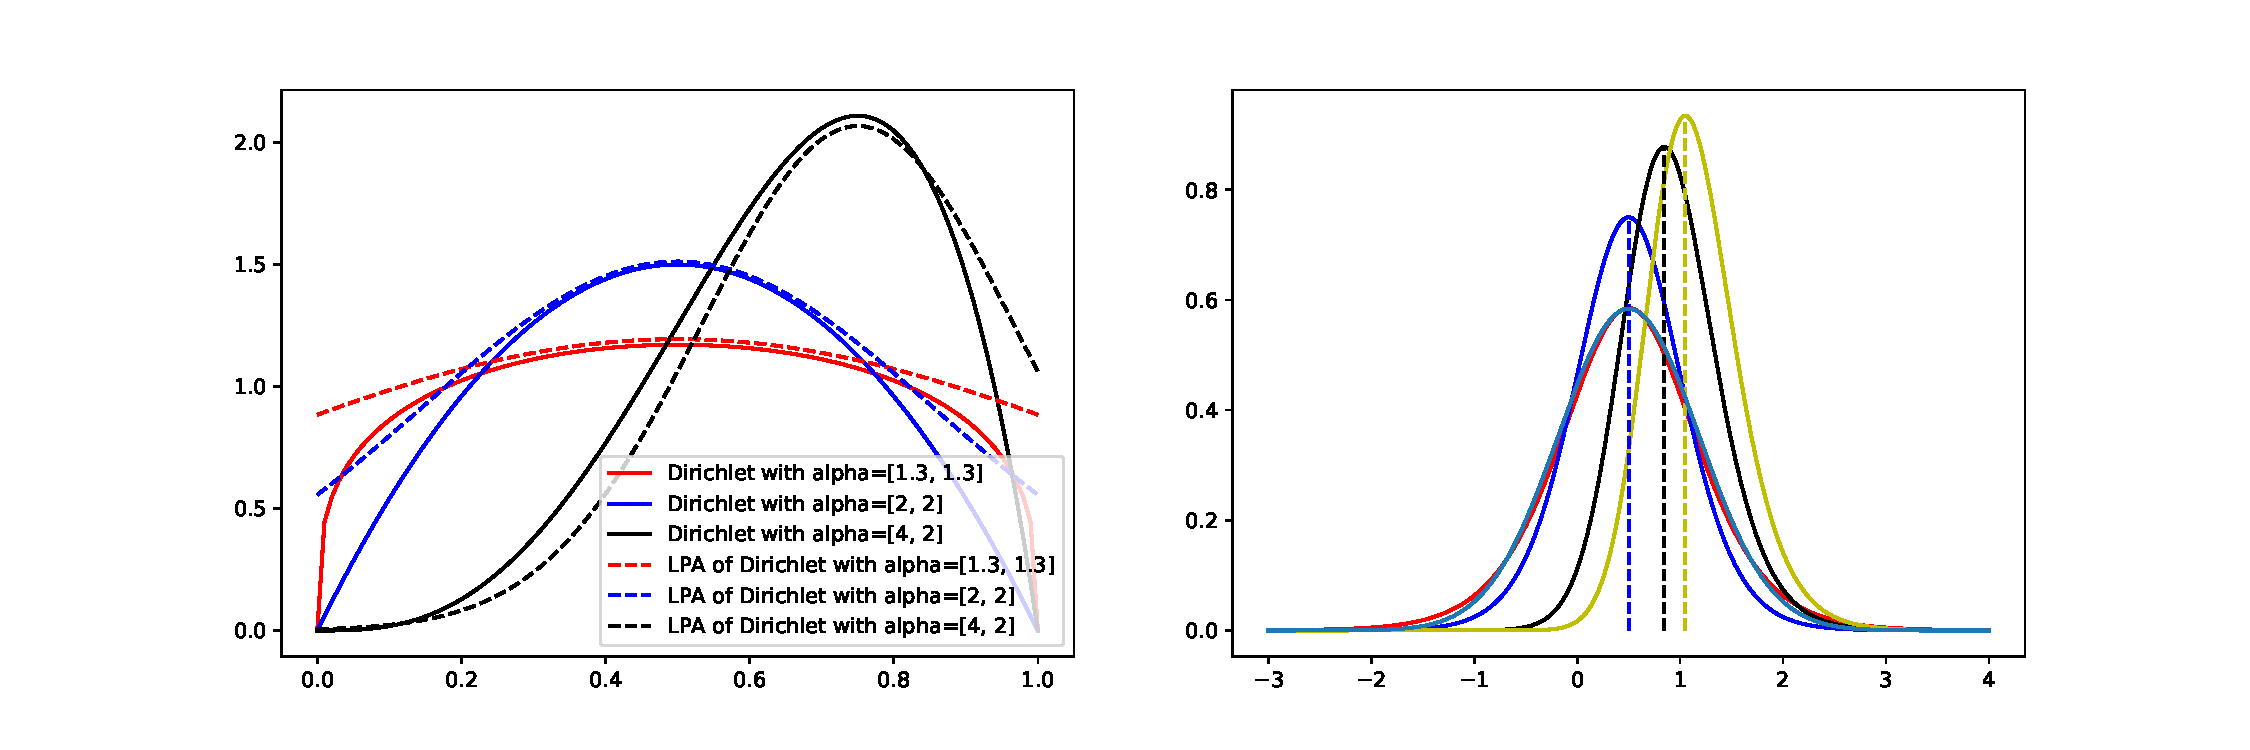
\includegraphics[width=\textwidth]{dirichlet_playground.pdf}
	\caption{Dirichlet comparison}
	\label{fig:Dirichlet_comparison}
\end{figure}

\section{Gamma Distribution}

\subsection{Standard Gamma Distribution}

\subsubsection{PDF of the Gamma Distribution}

\begin{equation}
	f(x, \alpha, \lambda) = \frac{\lambda^\alpha}{\Gamma(\alpha)} \cdot x^{(\alpha - 1)} \cdot e^{(-\lambda x)}
\end{equation}

where $\Gamma(\alpha)$ is the Gamma function. (DO I NEED TO EXPLAIN WHAT THAT IS?)

\subsubsection{Laplace Approximation of the Gamma Distribution}

To get the LPA of the Gamma function in the standard basis we need its mode and the second derivative of the log-pdf. The mode is already known to be $\hat{\theta} = \frac{\alpha -1}{\lambda}$. For the second derivative of the log-pdf we take the log-pdf and derive it twice and insert the mode for $x$:
\begin{align*}
	\text{log-pdf: } &\log\left( \frac{\lambda^\alpha}{\Gamma(\alpha)} \cdot x^{(\alpha - 1)} \cdot e^{(-\lambda x)}\right) \\
	&= \alpha \cdot \log(\lambda) - \log(\Gamma(\alpha)) + (\alpha -1)\log(x) -\lambda x\\
	\text{1st derivative: }& \frac{(\alpha-1)}{x} - \lambda \\
	\text{2nd derivative: }& \frac{(\alpha-1)}{x^2}\\
	\text{insert mode: }& \frac{(\alpha-1)}{(\frac{\alpha -1}{\lambda})^2} = \frac{\lambda^2}{\alpha - 1} \\
	\text{invert: }&\sigma^2 = \frac{\alpha-1}{\lambda^2}
\end{align*}

The LPA of the Gamma distribution is therefore approximately distributed according to the pdf of $N(\frac{\alpha - 1}{\lambda}, \frac{\lambda^2}{\alpha-1})$.

\subsection{Log-Transform of the Gamma Distribution}

\subsubsection{Log-Transformation}

We transform the Gamma Distribution with the Log-Transformation, i.e. $Y = \log(X)$. The pdf of the transformed Gamma Distribution is therefore distributed according to
$$f_Y(y) = f_X(\exp(y)) \cdot \left | \frac{d \exp(y)}{dy} \right|$$
as reasoned in Subsection \ref{subsec:variable_change_pdf}.

\subsubsection{PDF of the log-transformed Gamma Distribution}

The new pdf therefore becomes:

\begin{align}
f_t(x, \alpha, \lambda) &= \frac{\lambda^\alpha}{\Gamma(\alpha)} \cdot \exp(x)^{(\alpha - 1)} \cdot e^{(-\lambda \exp(x))} \cdot \exp(x) \\
&=\frac{\lambda^\alpha}{\Gamma(\alpha)} \cdot \exp(x)^{\alpha} \cdot e^{(-\lambda \exp(x))}
\end{align}

\subsubsection{Laplace Approximation of the log-transformed Gamma Distribution}

To get the LPA of the Gamma distribution in the (IS IT NOW EXP OR LOG BASIS?) we need to calculate its mode and the second derivative of the log-pdf. To get the mode we take the first derivative and set it to zero. 

\begin{align*}
\text{log-pdf: } &\log\left(\frac{\lambda^\alpha}{\Gamma(\alpha)} \cdot \exp(x)^{\alpha} \cdot exp(-\lambda \exp(x)) \right) \\
&= \alpha \log(\lambda) - \log(\Gamma(\alpha)) + \alpha x - \lambda \exp(x)\\
\text{1st derivative: }&  \alpha - \lambda \exp(x)\\
\text{mode: }& \alpha - \lambda \exp(x) = 0 \Leftrightarrow x = \log\left(\frac{\alpha}{\lambda}\right)\\
\text{2nd derivative: }&  -\lambda \exp(x)\\
\text{insert mode: }& -\lambda \exp(\log\left(\frac{\alpha}{\lambda}\right)) = -\frac{1}{\alpha} \\
\text{invert and times -1: }&\sigma^2 = \alpha 
\end{align*}

Therefore the LPA now is $N(\log\left(\frac{\alpha}{\lambda}\right), \alpha)$.

\subsection{Comparison}

plots and some measure to show similarity of two distributions

\begin{figure}[!htb]
	\centering
	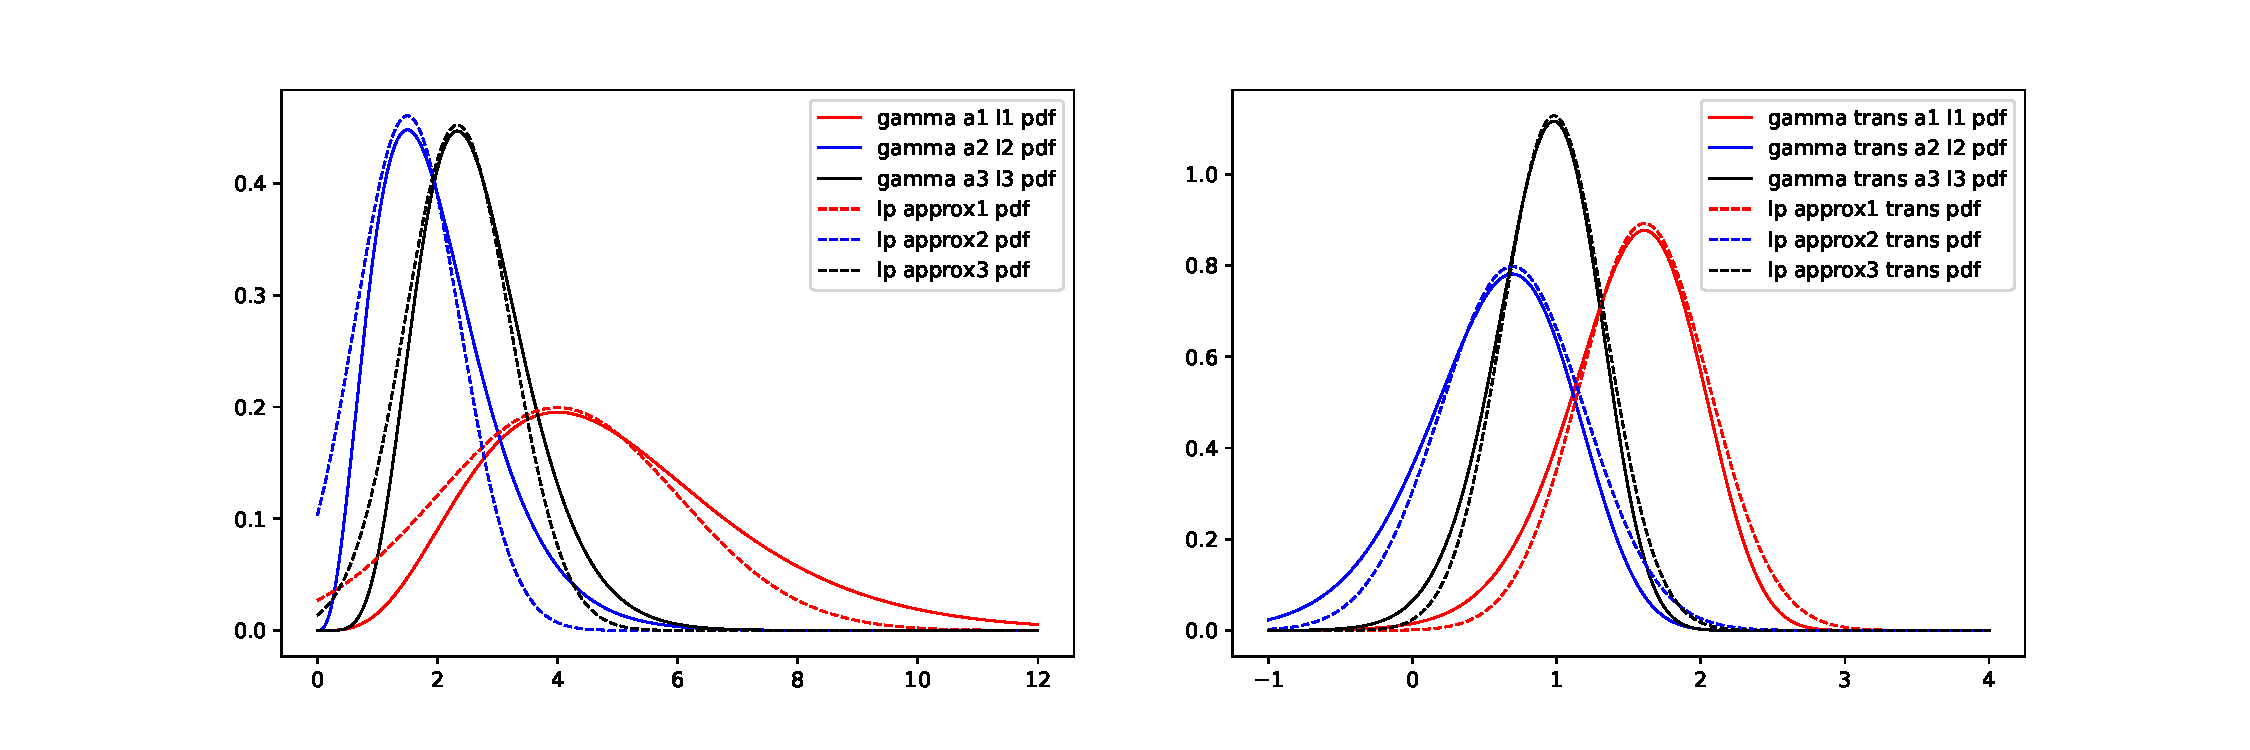
\includegraphics[width=\textwidth]{gamma_playground.pdf}
	\caption{gamma comparison}
	\label{fig:gamma_comparison}
\end{figure}

\section{Beta Distribution}

\subsection{Standard Beta Distribution}

\subsubsection{Pdf of the Beta Distribution}

\begin{align}
	f(x, \alpha, \beta) &= \frac{x^{(\alpha - 1)} \cdot (1-x)^{(\beta-1)}}{B(\alpha, \beta)} \\
	\text{with }B(\alpha, \beta) &= \frac{\Gamma(\alpha)\Gamma(\beta)}{\Gamma(\alpha + \beta)}
\end{align}

where $\Gamma(x)$ is the Gamma function.

\subsubsection{Laplace approximation of the Beta distribution}

TODO: explain stuff

\begin{align*}
\text{log-pdf: } &\log\left( \frac{x^{(\alpha - 1)} \cdot (1-x)^{(\beta-1)}}{B(\alpha, \beta)} \right) \\
&= (\alpha-1) \log(x) + (\beta-1)\log(1-x) - \log(B(\alpha,\beta)))\\
\text{1st derivative: }& \frac{(\alpha-1)}{x} - \frac{(\beta-1)}{1-x}  \\
\text{mode: }& \frac{(\alpha-1)}{x} - \frac{(\beta-1)}{1-x}  = 0 \Leftrightarrow x = \frac{\alpha-1}{\alpha + \beta - 2} \\
\text{2nd derivative: }& \frac{\alpha -1}{x^2} + \frac{\beta - 1}{(1 - x)^2} \\
\text{insert mode: }& \frac{\alpha -1}{\frac{\alpha-1}{\alpha + \beta - 2}^2} + \frac{\beta - 1}{(1 - \frac{\alpha-1}{\alpha + \beta - 2})^2} = \frac{(\alpha + \beta - 2)^3}{(\alpha-1)(\beta-1)}\\
\text{invert: }& \frac{(\alpha -1)(\beta-1)}{(\alpha + \beta - 2)^3}
\end{align*}

TODO: full derivations of mode and second derivative in appendix

The Beta distribution in standard basis is therefore approximated by $N(\mu = \frac{\alpha-1}{\alpha + \beta - 2}, \sigma^2 = \frac{(\alpha -1)(\beta-1)}{(\alpha + \beta - 2)^3})$.

\subsection{Logit-Transform of the Beta distribution}

\subsubsection{Logit-Transform}

using $g(x) = \log(\frac{x}{1-x})$. Therefore $g^{-1}(x) = \sigma(x) = \frac{1}{1+ \exp(-x)}$. 

\subsubsection{Pdf after logit transform}

\begin{align*}
	f_t(x, \alpha, \beta) &= \frac{\sigma(x)^{(\alpha - 1)} \cdot (1 - \sigma(x)^{(\beta -1)})}{B(\alpha, \beta)} \cdot (\sigma(x)(1-\sigma(x)) \\
	&=  \frac{\sigma(x)^{\alpha} \cdot (1 - \sigma(x)^{\beta})}{B(\alpha, \beta)}
\end{align*}

\subsubsection{LPA of the logit distribution after transform}

mode and variance of log pdf blablabla

\begin{align*}
\text{log-pdf: } &\log\left( \frac{\sigma(x)^{\alpha} \cdot (1 - \sigma(x)^{\beta})}{B(\alpha, \beta)} \right) \\
&= \alpha \log(\sigma(x)) + \beta \log(1 - \sigma(x)) - \log(B(\alpha, \beta))\\
\text{1st derivative: }&  \alpha (1 - \sigma(x)) - \beta \sigma(x)\\
\text{mode: }& \alpha (1 - \sigma(x)) - \beta \sigma(x) = 0 \Leftrightarrow x = -\log(\frac{\beta}{\alpha}) \\
\text{2nd derivative: }& (\alpha + \beta)\sigma(x)(1 - \sigma(x))  \\
\text{insert mode: }& (\alpha + \beta)\sigma(-\log(\frac{\beta}{\alpha}))(1 - \sigma(-\log(\frac{\beta}{\alpha}))) = \frac{\alpha\beta}{\alpha + \beta}  \\
\text{invert: }& \frac{\alpha + \beta}{\alpha \beta}
\end{align*}

TODO: full derivations of mode and second derivative in appendix

The LPA is therefore $N(\mu=-\log(\frac{\beta}{\alpha}), \sigma^2 = \frac{\alpha + \beta}{\alpha \beta})$.

\subsection{Comparison}

TODO: KL-Divergence or something similar

\begin{figure}[!htb]
	\centering
	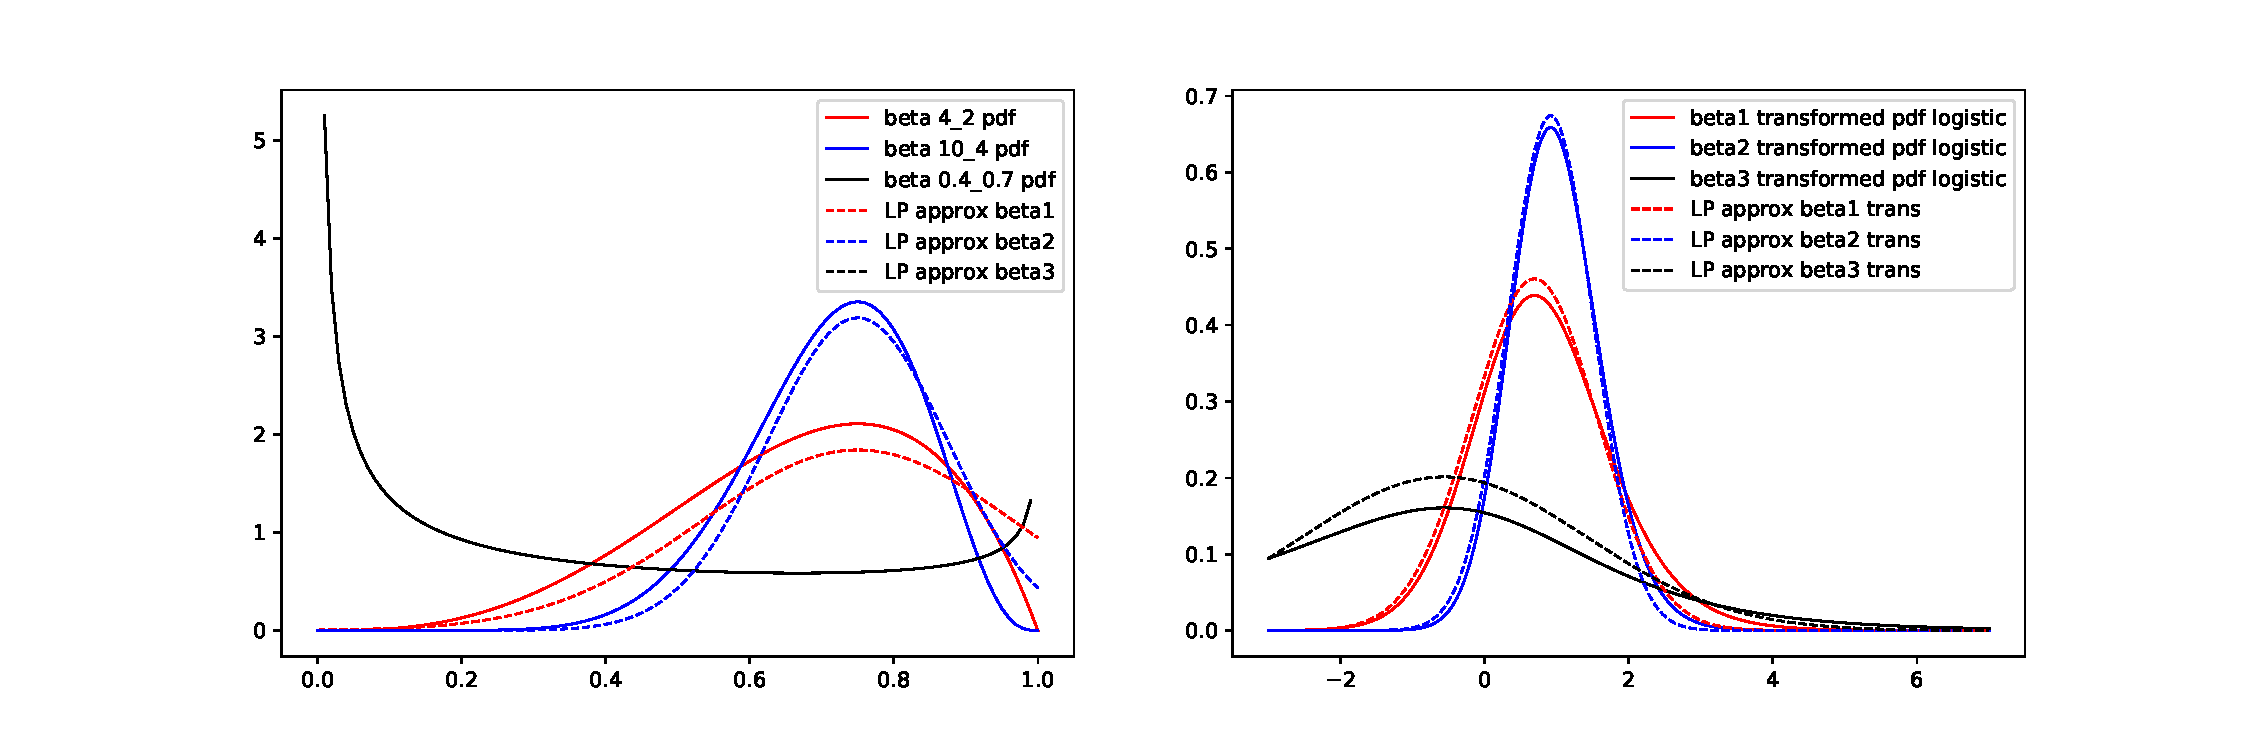
\includegraphics[width=\textwidth]{beta_playground.pdf}
	\caption{beta comparison}
	\label{fig:beta_comparison}
\end{figure}

\section{Chi-squared Distribution}

TODO: write up all

\begin{figure}[!htb]
	\centering
	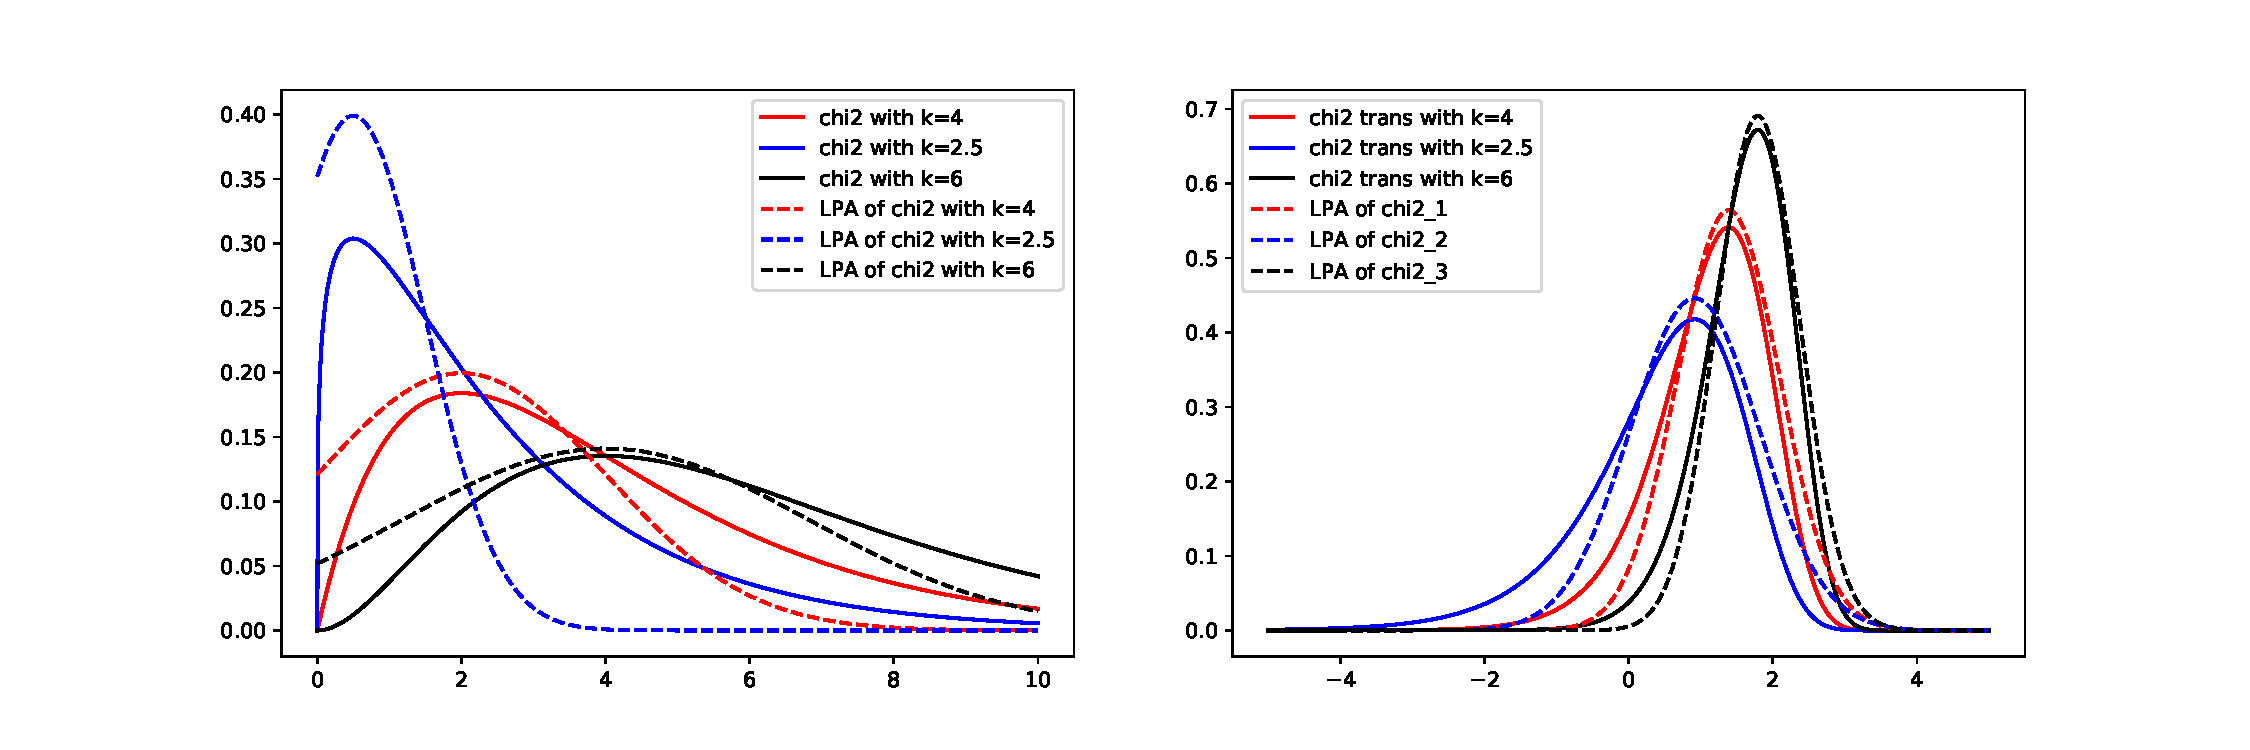
\includegraphics[width=\textwidth]{chi2_playground.pdf}
	\caption{chi2 comparison}
	\label{fig:chi2_comparison}
\end{figure}

\section{Wishart Distribution}

TODO: get the LPA of standard base and transformed base

\begin{figure}[!htb]
	\centering
	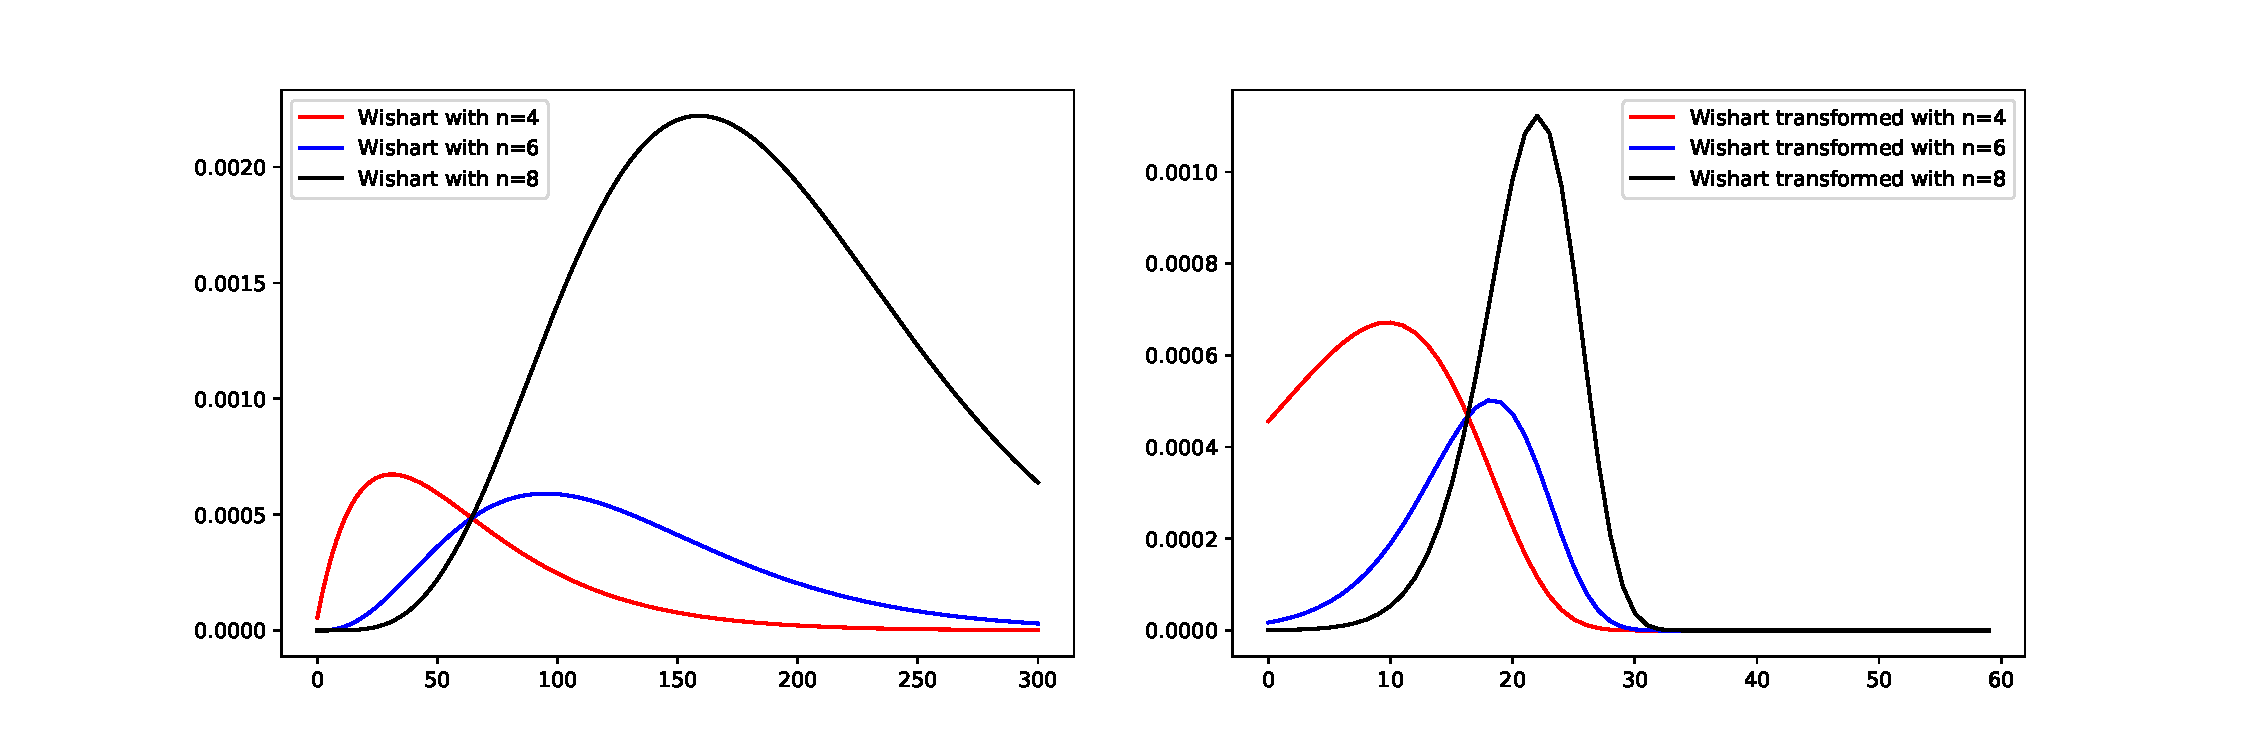
\includegraphics[width=\textwidth]{wishart_playground.pdf}
	\caption{wishart comparison}
	\label{fig:wishart_comparison}
\end{figure}

\section{Inverse Wishart Distribution}

TODO: see above

\begin{figure}[!htb]
	\centering
	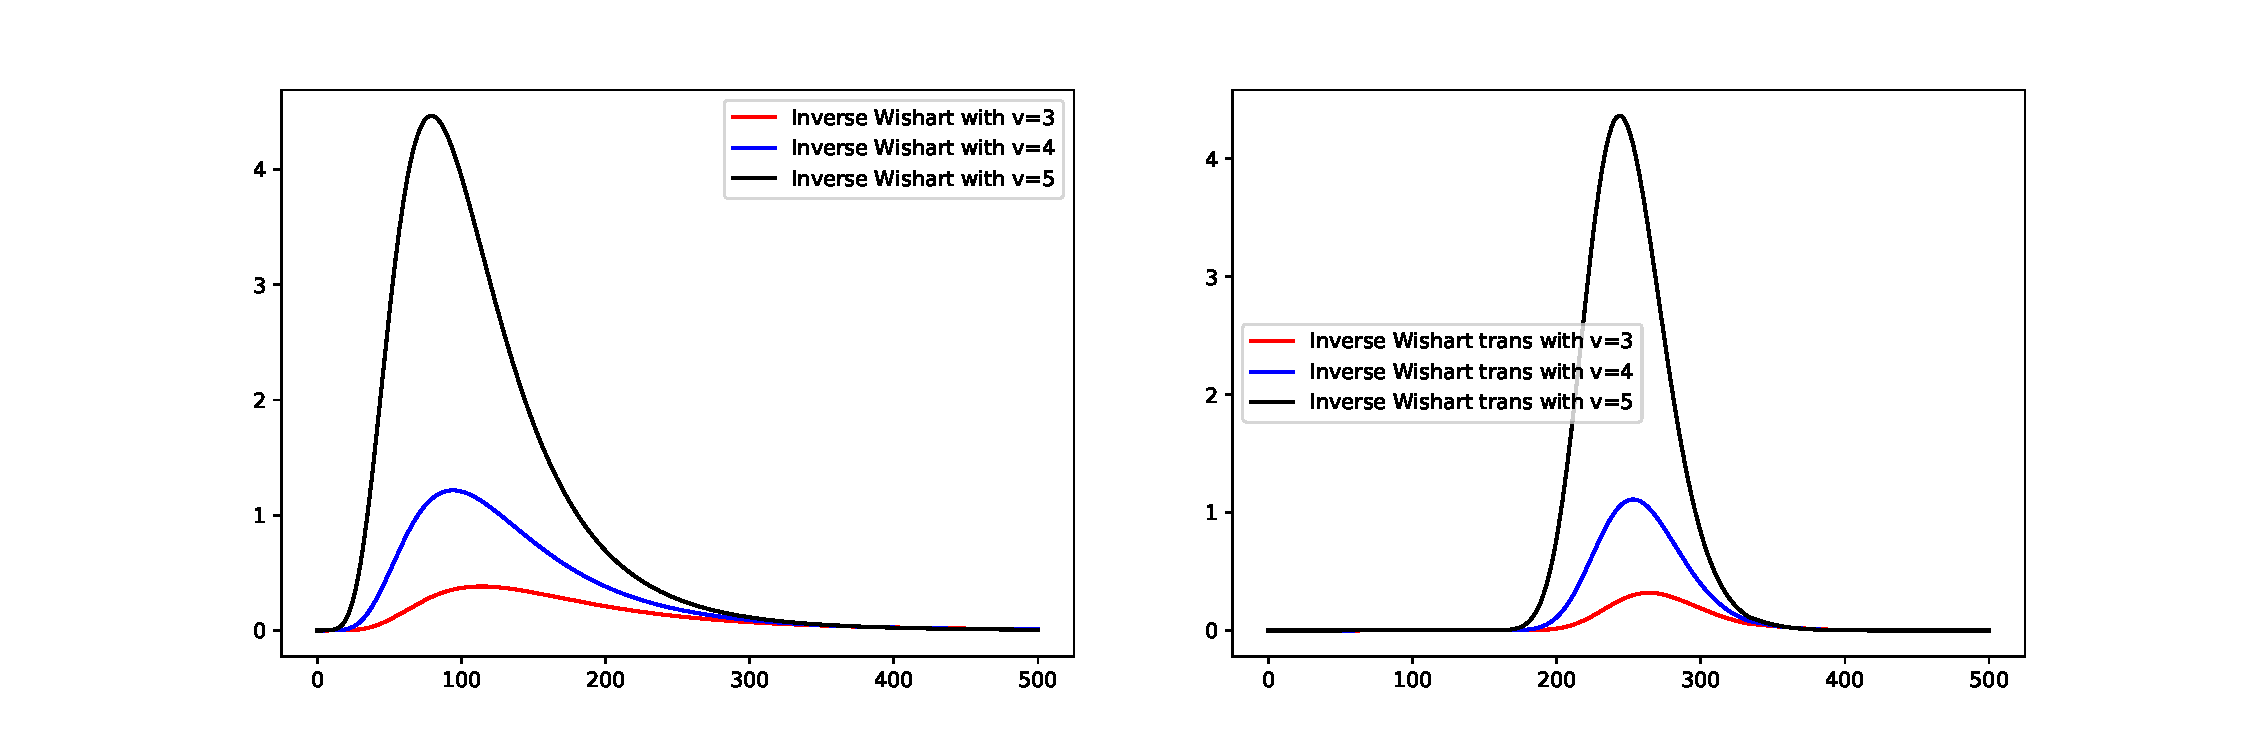
\includegraphics[width=\textwidth]{inverse_wishart_playground.pdf}
	\caption{inverse wishart comparison}
	\label{fig:inverse_wishart_comparison}
\end{figure}

\end{document}
